% !TeX spellcheck = en_US
\documentclass[a4paper]{scrartcl}
\usepackage[left=2cm, right=2cm, top=2cm, bottom=2cm]{geometry}
\usepackage{lmodern}
\usepackage[T1]{fontenc}
\usepackage[utf8]{inputenc}
\usepackage[english]{babel}
\usepackage{tabularx}
\usepackage{xcolor}
\usepackage{dirtree}
\usepackage[hidelinks]{hyperref}
\usepackage{algpseudocode}
\usepackage{algorithm}
\usepackage{algorithmicx}
\usepackage{tikz}
\usetikzlibrary{automata, positioning, arrows, shapes.geometric}

\newcommand{\file}[1]{\texttt{#1}}
\newcommand{\program}[1]{\textbf{#1}}
\newcommand{\variable}[1]{'\texttt{#1}'}
\newcommand{\module}[1]{\texttt{#1}}

\newcommand{\green}[1]{\textcolor{green}{#1}}

\title{Version 2 of the TSClient LEGACY Package Manager}
\subtitle{Developer's documentation}
\author{Thomas Erbesdobler <t.erbesdobler@gmx.de>}

\begin{document}
	\maketitle
	\tableofcontents
	
	
	\section{Introduction}
	\label{sec:introduction}
	
	Over the last two years (it's spring 2020) TSClient LEGACY has improved a lot. Though I cannot show you something yet. But the new build system requires a better package manager. Not that the TPM would be bad, but it's simply too slow and, most important as the time of this writing, does not allow to install packages when their files are already present. This makes it harder to bootstrap a system. I.e. one would have to install the bootstrapping toolchain into a different directory and adapt it after installing the final dynamic linker so that the compiler uses this one and lets the INTERP program header point to the correct interpreter.
	
	I think bootstrapping a system on the fly would be pretty cool, and hence I decided to rewrite the TPM in C++. I actually knew right after a few days working on and using the original TPM that I will have to do this one day, when I'll reach the limits of my Ocaml code as well as of the xml-based package database. So the primary new features that should come with this rewrite are the following (and I wanted all of them back then):
	
	\begin{itemize}
		\item A faster package database. Namely I'm going to use Sqlite3.
		\item The ability to adopt existing files. Not sure if this was the original plan back then, but I always felt like I need a better way to find conflicting packages than checking if their files are already in place before unpacking them.
		\item Source package version numbers shall be supported by the package manager. I always want it to be as slim as possible and not getting bloated with other stuff a package manager should not handle, but this seems very essential. Especially as the binary version numbers are difficult to understand in the context of microversioning. And I definitely don't want to end up doing something like \textit{"openssl-1.0.1h-2020.48.3097623"}.
		\item Truly support moving files between packages and therefore truly support conflicting packages. That is somewhat linked with adopting existing files as it requires the common base: conflicting packages.
		\item Not sure but I don't think the Ocaml code is exactly bleeding edge fast.
		\item More maintainer scripts (borrowed that term from Debian) and a more sensible way of using them (look at what rpm / dpkg does ...).
	\end{itemize}

	So, this document will contain the developer's documentation. That is especially internals and design decisions, but most important algorithms, concepts and maybe file formats, and a lot more if it comes into my vision.
	
	
	\section{depres}
	\label{sec:depres}
	
	First, I would like to talk about \module{depres}, which is the module that handles dependency resolution. The core of it is the dependency resolving algorithm, let me call it the depres-algorithm. It's input is a set of installed packages and a set of new packages that should be installed. It then constructs an installation graph from that through adding missing dependencies of the packages and choosing versions of packages to install. As second optimization goal apart from finding a feasible configuration of package versions such that all dependencies are fulfilled it tries to minimize the number of packages that need to be upgraded or installed. This distinguishes the conventional depres-algorithm from one used for upgrading all packages, which of course tries to maximize the number of upgraded packages.
	
	Before talking about the algorithm it is probably a good idea to explain my notion of dependencies.
	
	
	\subsection{Dependencies and dependency lists}
	\label{ssec:dependencies_and_dependency_lists}
	
	A dependency is a pair of the package (name and architecture) on which shall be depended and a predicate that constrains the accepted versions of that package. This is usually a predicate-logical formula made of and- and or connected less-/bigger-/equal predicates on the destination package's version. Practically I would implement this as a struct (or class; it's the same in C++ anyway) with the name as member and maybe a list of lists that represents the formula in CNF or DNF. Maybe I could also translate an arbitrary formula to objects representing and- and or operators by objects that have two children and so on. The former is probably easier (actually faster) to verify against a given version number because not the entire syntax tree of the formula needs to be parsed. But the latter could be easier to maintain, given that usually during parsing the packed form of a package constraints are only added and not deleted. One thing is however clear: the latter cannot be represented by vectors. Anyway, I'll see.
	
	Such a dependency describes one package to depend on. Now a dependency list is simply a list of such dependencies with each describing a different package. I don't think it must be anything special as no lookups will probably be done in that list. As there are binary- and source version dependencies, a package's dependencies can be described by two lists.
	
	Having said that I can now talk about the depres-algorithm.
	
	
	\subsection{The depres-algorithm}
	\label{ssec:the_depres_algorithm}
	
	It's probably similar to the original depres-algorithm used in the original TPM's depres \module{depres} module.
	
	The algorithm maintains an installation graph and a set of 'active' packages. A package is 'active' if it's version is not decided upon yet and/or its dependencies were not added to the graph yet. This can also mean that a version has been chosen but the algorithm did not yet verify if it still fulfills the requirements. The installation graph's nodes represent packages in two different states: installed already or to be installed / upgraded. Additionally if the algorithm installs a package, it stores why it decided to do so to distinguish between automatically- and manually installed packages. Each node is annotated with the currently chosen package version and predicate that specifies the accepted versions of that package. It's similar to the one used for dependencies, but each sub-predicate needs to be annotated with the package that imposed it. Therefore using a conjunction of multiple clauses is better here because each clause can then be attributed to a package. It is important to store that information as the requirements of packages may change as they are upgraded. That means removing old dependencies and adding new ones.
	
	Installing and upgrading packages can introduce conflicting packages into the system. I think the package manager should be able to deal with them as long as older or automatically installed packages will or can be removed during installation. This begs the question when these packages should be removed. I would say just before the conflicting packages will be installed to keep them as long as possible. This requires unconfiguring them and removing files that will not be overwritten by the new package. Other files should be kept to allow a smooth transition. However I'm pretty sure that this is not enough and removing manually installed packages needs to be allowed, too. Consider i.e. packages A and B that do not conflict. Now there is a new package C that replaces both. A and B may be manually installed ...
	
	Initially the installation graph is empty. The algorithm adds all installed packages and their version numbers. It adds all dependencies of the installed packages as edges and to the packages' formulas. After that the installation graph represents the current situation. I can do a check if the configuration is valid by verifying that the chosen versions fulfill the formulas and they do not conflict, and abort early if that's not the case, leaving the residing work to a repair operation.
	
	Then all requested packages are added to the graph as nodes, but not their dependencies. And the algorithm adds them to the set of active packages. Now while the set is not empty, remove a package from it and locate it in the graph. If no specific version is chosen yet or if the chosen version does not fulfill the formula, add all its dependencies by introducing new edges to existing packages or finding and adding new packages to the graph that are not installed yet. The latter's dependencies don't need to be considered yet. The current package's however are added to the constraint lists as well. And every dependency is added to the set of active packages as it's version constraining formula might have changed. After all the resulting installation graph represents a feasible situation because every dependency and every constraint that goes with them was added to the graph and every package was checked against these constraints at least once.
	
	The algorithm's running time is at least $\mathcal{O}(n)$ with number of packages as $n$ since all considered packages need to be added to the graph. Moreover the algorithm performs multiple rounds until the set of installed packages is empty. I prefer a deterministic set datastructure here, hence every set-operation will be $\mathcal{O}(\log{}n)$. In each round a package is removed and all its dependencies are added if and only if the package did not fulfill the imposed version formula. This leads to an exponential running time. In practice however I think it will be rarely the case that multiple versions need to be tried. If the first version suffices for each package, each package will never be added to the set again after having been removed \textbf{and} after all packages are in the graph. So when a package is added the set may grow to size $\mathcal{O}(n)$ again. This can happen $\mathcal{O}(n)$ times leading to a practical running time of $\mathcal{O}(n^2)$, but with super-exponential worst case if all versions need to be tried and the number of versions is linear in the number of packages (could happen as both may be linear in lifetime).
	
	\paragraph{Removing conflicting packages} Whenever a (not already installed) package is added to the installation graph it may conflict with another one. I have to check that with every package (does not increase already quadratic running time) and remove the ones that conflict with the package as well as their dependency-edges and their constraint predicates in the version constraining formulas. A message to the user that can optionally be ignored would be nice. Add all reverse dependencies to the set of active packages. Then, whenever a package is removed from that set and processed in a round, it could bring the old package back (unless there is an 'or'-dependency). The algorithm can try a different version, especially as newer versions may have updated dependencies that reflect the newer package base that in turn created that conflict with packages from an older base, but if that fails it must abort when it recognizes that the situation cannot be solved as long as a certain new package needs to be installed.
	
	So different versions of all packages that depend on a removed one potentially need to be tried again and therefore all these packages need to be added to the set. This can be done by starting a DFS at the removed package that traverses edges in reverse direction. To make this work the algorithm needs to try different versions first before declaring a conflict.
	
	
	\vspace{1eM}
	Before I try further things I want to make the algorithm more concrete.
	
	\begin{algorithm}[ht]
		\caption{Pseudo code of the depres-algorithm}
		\label{alg:pseudo_code_of_the_depres_algorithm}
		
		\begin{algorithmic}
			\State $active\gets \emptyset$
			\State $V\gets \emptyset$
			\State $E\gets \emptyset$
			\State $G\gets (V, E)$
			
			\For{$p\in installed\_packages$}
				\State $V\gets V\cup \{p\}$
			\EndFor
				
			\For{$p\in installed\_packages$}
				\For{$d\in p.dependencies$}
					\State $E\gets E\cup \{(p,d)\}$
				\EndFor
			\EndFor
			\State $\vdots$
		\end{algorithmic}
	\end{algorithm}


	\subsection{Pre-dependencies vs. dependencies}
	\label{sec:pre_dependencies_vs_dependencies}
	
	There are two flavors of dependencies between packages. The more usual dependencies declare required packages at configure stage, while the dependencies need not be fulfilled during the preinst script and extracting. That means packages can be extracted and their preinst script be run in any order and the package manager ensures that dependencies are met only for configuration and later installed packages. A preinst script however could require other packages, too. It usually will at least need an interpreter, therefore requiring a dependency facility before a package's installation begins. The TPM2 achieves this (like Debian's dpkg and rpm) through pre-dependencies. They are handles in the same way like regular dependencies but ensured before the preinst script is run. Of course cycles here must be broken at a point and hence cannot be fulfilled.
	
	There is one more important case that I would like to note here: pre-dependencies could require the same package as regular dependencies. But the required version must be the same, otherwise the package manager would have to change a dependency's version during the installation of the dependent package. I can't think of a legitimate use case for this, and avoiding that makes things easier. The installation graph needs only one set of nodes.
	
	Additionally pre-dependencies should also be available to the postrm script as the package is not configured anymore when the package manager runs it. Hence it is probably a good idea to keep them while the depending package is installed to avoid having to install another package first before a package can be uninstalled.
	
	
	\section{PackageDB}
	\label{sec:packagedb}
	
	''\module{PackageDB}'' or ''\module{package\_db}'' is the package manager's database, which stores the installed packages, their states and which files are installed. The latter is especially interesting since one has to decide which attributes of files to store. For now I decided to use the following simple schema:
	
	\begin{table}[H]
		\centering
		
		\begin{tabular}{ll}
			schema\_version: & \underline{version:varchar} \\
			packages: & \underline{name:varchar}, \underline{arch:integer}, \underline{version:varchar}, state:int, source\_version:varchar \\
			files: & \underline{path:varchar}, \underline{pkg\_name:varchar}, \underline{pkg\_arch}, \underline{version:varchar}, digest:varchar \\
		\end{tabular}
	
		\caption{The database schema of \module{PackageDB}}
		\label{tab:the_database_schema_of_packagedb}
	\end{table}
	
	It does not store file attributes at all. This deviates from the aforementioned ideal of a package manager which knows all files, but makes the implementation easier. At least for now I don't see why having the stricter version could bring a big benefit in my current and mid-term practice. If that arises it can easily be added due to versioned db schemata, anyway. The digest field contains a hash of the file's content. It may be prefixed with something like ''\texttt{sha512:}'' to indicate the used algorithm. If not prefix is present, the algorithm shall be sha1. It's not like super-safety but a considerable measure of integrity protection.
	
	
	\section{Package states}
	\label{sec:package_states}
	
	At any point in time a package that is part of the system has a state. This state describes if it is fully part of the system or in a, say, transitional state, where the package manager needs to do more work until the package's invariants are fulfilled. State transitions are atomic operations of the package manager. As such, these must be idempotent to allow for repeating them if they were interrupted. Figures \ref{fig:package_states_install}, \ref{fig:package_states_remove} and \ref{fig:package_states_change} describe the possible state transitions and which actions go with them when installing, removing or changing a package. The latter needs to consider the old and the new version of a package. ''change'' refers to upgrading or downgrading. As a package's files may be replaced by multiple packages or multiple packages' files may be consumed by one package, this is the most complicated procedure and it involves more than one package.
	
	In other words, as long as no conflicting packages are part of the system it's easy. Conflicting packages can be there in transient states, however not in an accepted state (i.e. configured).
	
	\begin{figure}[ht]
		\centering
		
		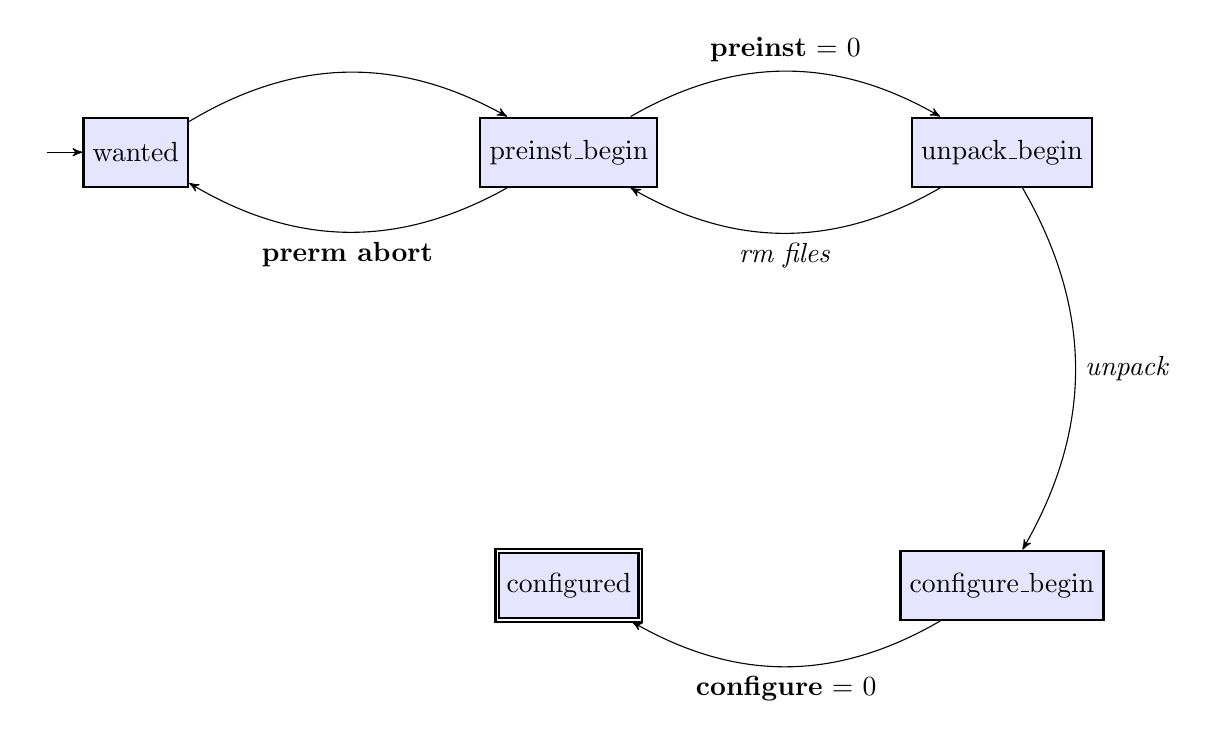
\begin{tikzpicture}[
				->,
				>=stealth',
				node distance=5.5cm,
				every state/.style={thick, fill=blue!10, rectangle},
				initial text=$ $]
			
			\node[state, initial] (wanted) {wanted};
			\node[state, right of=wanted] (preinst_begin) {preinst\_begin};
			\node[state, right of=preinst_begin] (unpack_begin) {unpack\_begin};
			\node[state, below of=unpack_begin] (configure_begin) {configure\_begin};
			\node[state, accepting, left of=configure_begin] (configured) {configured};
			
			\draw	(wanted) edge[above, bend left] node{$ $} (preinst_begin)
					(preinst_begin) edge[above, bend left] node{\program{preinst} = 0} (unpack_begin)
					(unpack_begin) edge[right, bend left] node{\textit{unpack}} (configure_begin)
					(configure_begin) edge[below, bend left] node{\program{configure} = 0} (configured);
					
			\draw 	(preinst_begin) edge[below, bend left] node{\program{prerm abort}} (wanted)
					(unpack_begin) edge[below, bend left] node{\textit{rm files}} (preinst_begin);
			
			
		\end{tikzpicture}
		
		\caption{Package states during installation}
		\label{fig:package_states_install}
	\end{figure}

	The ''begin'' states are required to be undo operations only once they were started. Otherwise the package manager would i.e. have to run \program{unconfigure} again when in state unpacked, even though some files may have been removed already. \program{unconfigure} may fail then. It is not required for all states but then some operations have to redo work. That is not a problem since maintainer scripts must be idempotent anyway (consider the package manager was interrupted just before it committed to the db that a script was run). One can view the system not as having states as points in time where one operation ended and the next one will begin but one operation ended some time ago and the next one may have begun already. That indicates the direction that the last operation that induced a state change took and allows to restart from there after an interruption, only redoing this one operation rather than having to consider all directions. This limits idempotence to one operation and not one operation and its predecessor.
	
	I would not need that indication of direction if I only considered one process, like only install. But I always need at least both.
	
	The state ''wanted'' only exists because packages may lie around in memory while they're not installed yet and need to have a state. And because I did not want a tristate-like type for it. It does not need to be stored in the db.
	
	Table \ref{tab:required_package_states} summarizes the states a package can be in.
	
	\begin{table}[ht]
		\centering
		
		\begin{itemize}
			\item wanted
			\item preinst\_begin
			\item unpack\_begin
			\item configure\_begin
			\item configure
			\item unconfigure\_begin
			\item rm\_files\_begin
			\item postrm\_begin
		\end{itemize}
		
		\caption{Required package states}
		\label{tab:required_package_states}
	\end{table}
	
\end{document}